% Compression Algorithms - A Comprehensive Guide
% Author: Abdessamad JAOUAD
% Program: M2 Big Data & IoT, ENSAM Casablanca
% Date: January 2025

\documentclass[11pt,a4paper]{report}

% ============================================
% PACKAGES
% ============================================
\usepackage[utf8]{inputenc}
\usepackage[T1]{fontenc}
\usepackage{lmodern}
\usepackage[english]{babel}
\usepackage{geometry}
\geometry{margin=2.5cm}

% Graphics and colors
\usepackage{graphicx}
\usepackage{tikz}
\usetikzlibrary{shapes,arrows,positioning,calc,decorations.pathreplacing,patterns,fit,backgrounds}
\usepackage{pgfplots}
\pgfplotsset{compat=1.17}

% Tables
\usepackage{booktabs}
\usepackage{tabularx}
\usepackage{longtable}
\usepackage{multirow}
\usepackage{colortbl}
\usepackage{array}

% Math
\usepackage{amsmath}
\usepackage{amssymb}

% Code listings
\usepackage{listings}
\usepackage{algorithm}
\usepackage{algorithmic}

% Formatting
\usepackage{fancyhdr}
\usepackage{titlesec}
\usepackage{hyperref}
\usepackage{xcolor}
\usepackage{enumitem}

% Colors
\definecolor{primaryblue}{RGB}{0,82,147}
\definecolor{secondarygreen}{RGB}{0,150,100}
\definecolor{accentorange}{RGB}{255,127,0}
\definecolor{lightgray}{RGB}{245,245,245}
\definecolor{darkgray}{RGB}{80,80,80}

% Hyperref setup
\hypersetup{
    colorlinks=true,
    linkcolor=primaryblue,
    filecolor=primaryblue,
    urlcolor=primaryblue,
    citecolor=secondarygreen
}

% Header/Footer
\pagestyle{fancy}
\fancyhf{}
\fancyhead[L]{\leftmark}
\fancyhead[R]{Compression Algorithms}
\fancyfoot[C]{\thepage}
\renewcommand{\headrulewidth}{0.4pt}

% Chapter formatting
\titleformat{\chapter}[display]
{\normalfont\huge\bfseries\color{primaryblue}}
{\chaptertitlename\ \thechapter}{20pt}{\Huge}

% Code listing style
\lstdefinestyle{mystyle}{
    backgroundcolor=\color{lightgray},
    basicstyle=\ttfamily\small,
    breaklines=true,
    frame=single,
    numbers=left,
    numberstyle=\tiny\color{darkgray},
    keywordstyle=\color{primaryblue}\bfseries,
    commentstyle=\color{secondarygreen},
    stringstyle=\color{accentorange}
}
\lstset{style=mystyle}

% ============================================
% DOCUMENT
% ============================================
\begin{document}

% ============================================
% TITLE PAGE
% ============================================
\begin{titlepage}
\centering
\vspace*{2cm}

{\Huge\bfseries\color{primaryblue} Compression Algorithms\par}
\vspace{0.5cm}
{\Large\color{darkgray} A Comprehensive Guide\par}

\vspace{2cm}

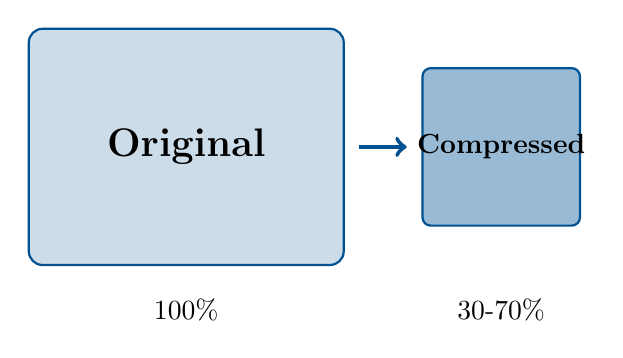
\begin{tikzpicture}
    % Main compression icon
    \draw[fill=primaryblue!20, draw=primaryblue, thick, rounded corners=5pt] (0,0) rectangle (4,3);
    \draw[fill=primaryblue!40, draw=primaryblue, thick, rounded corners=3pt] (5,0.5) rectangle (7,2.5);
    \draw[->, ultra thick, primaryblue] (4.2,1.5) -- (4.8,1.5);
    \node at (2,1.5) {\Large\textbf{Original}};
    \node at (6,1.5) {\textbf{Compressed}};
    \node[below] at (2,-0.3) {100\%};
    \node[below] at (6,-0.3) {30-70\%};
\end{tikzpicture}

\vspace{2cm}

{\Large\textit{RLE $\bullet$ Delta $\bullet$ Huffman $\bullet$ LZ77/LZ78 $\bullet$ LZW}\par}
{\Large\textit{DEFLATE $\bullet$ LZ4 $\bullet$ Zstandard $\bullet$ Brotli $\bullet$ bzip2}\par}

\vfill

{\large Abdessamad JAOUAD\par}
{\normalsize M2 Big Data \& IoT\par}
{\normalsize ENSAM Casablanca\par}

\vspace{1cm}
{\normalsize January 2025\par}
\end{titlepage}

% ============================================
% TABLE OF CONTENTS
% ============================================
\tableofcontents
\newpage

% ============================================
% CHAPTER 1: INTRODUCTION
% ============================================
\chapter{Introduction to Data Compression}

\section{What is Data Compression?}

\textbf{Data compression} is the process of reducing the number of bits needed to represent data. This reduction allows for:
\begin{itemize}[itemsep=5pt]
    \item \textbf{Storage savings}: Store more data in the same space
    \item \textbf{Faster transmission}: Send data more quickly over networks
    \item \textbf{Reduced costs}: Lower storage and bandwidth expenses
\end{itemize}

\begin{figure}[h]
\centering
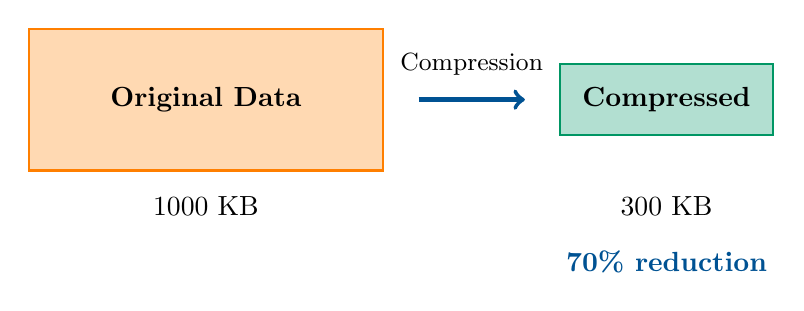
\begin{tikzpicture}[scale=0.9]
    % Original data
    \draw[fill=accentorange!30, draw=accentorange, thick] (0,0) rectangle (5,2);
    \node at (2.5,1) {\textbf{Original Data}};
    \node at (2.5,-0.5) {1000 KB};
    
    % Arrow
    \draw[->, ultra thick, primaryblue] (5.5,1) -- (7,1);
    \node[above] at (6.25,1.2) {\small Compression};
    
    % Compressed data
    \draw[fill=secondarygreen!30, draw=secondarygreen, thick] (7.5,0.5) rectangle (10.5,1.5);
    \node at (9,1) {\textbf{Compressed}};
    \node at (9,-0.5) {300 KB};
    
    % Ratio
    \node[below] at (9,-1) {\color{primaryblue}\textbf{70\% reduction}};
\end{tikzpicture}
\caption{The compression process reduces data size significantly}
\end{figure}

\section{Types of Compression}

\subsection{Lossless Compression}
Data is compressed without any loss of information. The original data can be perfectly reconstructed.

\textbf{Use cases}: Text files, executable programs, archives, databases

\textbf{Algorithms}: Huffman, LZW, DEFLATE, bzip2, LZMA

\subsection{Lossy Compression}
Some information is permanently discarded to achieve higher compression ratios.

\textbf{Use cases}: Images (JPEG), audio (MP3), video (H.264)

\begin{table}[h]
\centering
\begin{tabular}{lcc}
\toprule
\textbf{Aspect} & \textbf{Lossless} & \textbf{Lossy} \\
\midrule
Data Recovery & Perfect & Approximate \\
Compression Ratio & 2:1 to 10:1 & 10:1 to 100:1 \\
Use Case & Text, Code & Media \\
\bottomrule
\end{tabular}
\caption{Comparison of lossless and lossy compression}
\end{table}

\section{Key Concepts}

\subsection{Compression Ratio}
\begin{equation}
\text{Compression Ratio} = \frac{\text{Original Size}}{\text{Compressed Size}}
\end{equation}

A ratio of 3:1 means the compressed file is 1/3 the size of the original.

\subsection{Entropy}
Shannon entropy measures the theoretical minimum bits needed to encode data:
\begin{equation}
H(X) = -\sum_{i=1}^{n} p(x_i) \log_2 p(x_i)
\end{equation}
where $p(x_i)$ is the probability of symbol $x_i$.

\section{Classification of Algorithms}

\begin{figure}[h]
\centering
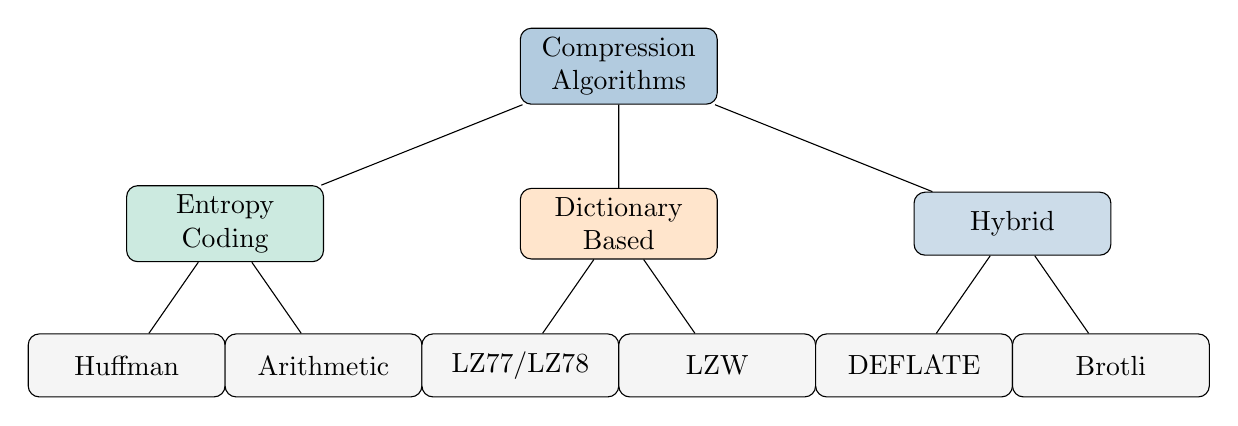
\begin{tikzpicture}[
    level 1/.style={sibling distance=50mm, level distance=20mm},
    level 2/.style={sibling distance=25mm, level distance=18mm},
    every node/.style={draw, rounded corners, fill=primaryblue!10, minimum width=2.5cm, minimum height=0.8cm, align=center}
]
\node[fill=primaryblue!30] {Compression\\Algorithms}
    child {node[fill=secondarygreen!20] {Entropy\\Coding}
        child {node[fill=lightgray] {Huffman}}
        child {node[fill=lightgray] {Arithmetic}}
    }
    child {node[fill=accentorange!20] {Dictionary\\Based}
        child {node[fill=lightgray] {LZ77/LZ78}}
        child {node[fill=lightgray] {LZW}}
    }
    child {node[fill=primaryblue!20] {Hybrid}
        child {node[fill=lightgray] {DEFLATE}}
        child {node[fill=lightgray] {Brotli}}
    };
\end{tikzpicture}
\caption{Classification of compression algorithms}
\end{figure}

% ============================================
% CHAPTER 2: RUN-LENGTH ENCODING
% ============================================
\chapter{Run-Length Encoding (RLE)}

\section{Overview}

\textbf{Run-Length Encoding} is one of the simplest compression algorithms. It replaces sequences of identical symbols (runs) with a count and the symbol.

\begin{itemize}
    \item \textbf{Type}: Lossless
    \item \textbf{Complexity}: $O(n)$ time and space
    \item \textbf{Best for}: Data with many consecutive repeated values
\end{itemize}

\section{How It Works}

\begin{figure}[h]
\centering
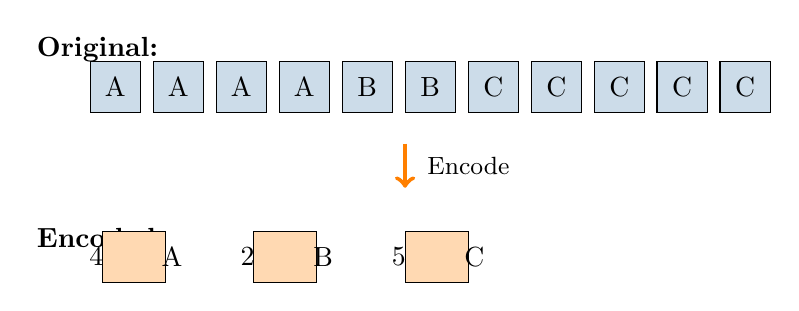
\begin{tikzpicture}[scale=0.8]
    % Original string
    \node[anchor=west] at (0,3) {\textbf{Original:}};
    \foreach \i/\c in {1/A,2/A,3/A,4/A,5/B,6/B,7/C,8/C,9/C,10/C,11/C} {
        \draw[fill=primaryblue!20] (\i,2) rectangle (\i+0.8,2.8);
        \node at (\i+0.4,2.4) {\c};
    }
    
    % Arrow
    \draw[->, ultra thick, accentorange] (6,1.5) -- (6,0.8);
    \node[right] at (6.2,1.15) {\small Encode};
    
    % Encoded string
    \node[anchor=west] at (0,0) {\textbf{Encoded:}};
    \foreach \i/\c in {1/4,2/A,3/2,4/B,5/5,6/C} {
        \ifodd\i
            \draw[fill=secondarygreen!30] (\i*1.2,-.7) rectangle (\i*1.2+1,0.1);
        \else
            \draw[fill=accentorange!30] (\i*1.2-1.2,-.7) rectangle (\i*1.2-0.2,0.1);
        \fi
        \node at (\i*1.2+0.5-0.6,-0.3) {\c};
    }
\end{tikzpicture}
\caption{RLE encoding: AAAABBCCCCC $\rightarrow$ 4A2B5C}
\end{figure}

\section{Algorithm}

\begin{algorithm}[H]
\caption{Run-Length Encoding}
\begin{algorithmic}[1]
\STATE \textbf{Input:} String $S$ of length $n$
\STATE \textbf{Output:} Encoded string
\STATE $result \gets$ empty string
\STATE $count \gets 1$
\FOR{$i = 1$ to $n-1$}
    \IF{$S[i] = S[i-1]$}
        \STATE $count \gets count + 1$
    \ELSE
        \STATE Append $count$ and $S[i-1]$ to $result$
        \STATE $count \gets 1$
    \ENDIF
\ENDFOR
\STATE Append $count$ and $S[n-1]$ to $result$
\RETURN $result$
\end{algorithmic}
\end{algorithm}

\section{Example}

\begin{table}[h]
\centering
\begin{tabular}{lccc}
\toprule
\textbf{Input} & \textbf{Output} & \textbf{Original} & \textbf{Compressed} \\
\midrule
WWWWWWWWWWWWBWWW & 12W1B3W & 16 chars & 7 chars \\
AABBBCCCC & 2A3B4C & 9 chars & 6 chars \\
ABCDEF & 1A1B1C1D1E1F & 6 chars & 12 chars (expansion!) \\
\bottomrule
\end{tabular}
\caption{RLE encoding examples}
\end{table}

\section{Advantages and Limitations}

\begin{table}[h]
\centering
\begin{tabular}{p{6cm}p{6cm}}
\toprule
\textbf{Advantages} & \textbf{Limitations} \\
\midrule
\textcolor{secondarygreen}{\textbullet} Very simple to implement & \textcolor{red}{\textbullet} Can expand data with few runs \\
\textcolor{secondarygreen}{\textbullet} Fast encoding/decoding & \textcolor{red}{\textbullet} Not effective for random data \\
\textcolor{secondarygreen}{\textbullet} No dictionary needed & \textcolor{red}{\textbullet} Limited compression ratio \\
\textcolor{secondarygreen}{\textbullet} Low memory usage & \textcolor{red}{\textbullet} Best only for specific data types \\
\bottomrule
\end{tabular}
\end{table}

\section{Applications}

\begin{itemize}
    \item \textbf{Fax transmission} (CCITT Group 3/4)
    \item \textbf{Bitmap images} (BMP, PCX, TIFF)
    \item \textbf{Icons and simple graphics}
    \item \textbf{PackBits} (used in TIFF)
\end{itemize}

% ============================================
% CHAPTER 3: DELTA ENCODING
% ============================================
\chapter{Delta Encoding}

\section{Overview}

\textbf{Delta encoding} stores differences between consecutive values rather than the values themselves. This is highly effective when consecutive values are similar.

\begin{itemize}
    \item \textbf{Type}: Lossless
    \item \textbf{Complexity}: $O(n)$
    \item \textbf{Best for}: Time series, sensor data, version control
\end{itemize}

\section{How It Works}

\begin{figure}[h]
\centering
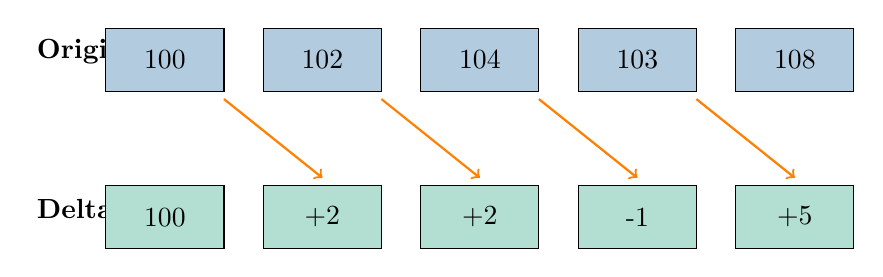
\begin{tikzpicture}
    % Original values
    \node[anchor=west] at (-1,2.5) {\textbf{Original:}};
    \foreach \i/\v in {0/100,1/102,2/104,3/103,4/108} {
        \draw[fill=primaryblue!30] (\i*2,2) rectangle (\i*2+1.5,2.8);
        \node at (\i*2+0.75,2.4) {\v};
    }
    
    % Delta values
    \node[anchor=west] at (-1,0.5) {\textbf{Delta:}};
    \foreach \i/\v in {0/100,1/+2,2/+2,3/-1,4/+5} {
        \draw[fill=secondarygreen!30] (\i*2,0) rectangle (\i*2+1.5,0.8);
        \node at (\i*2+0.75,0.4) {\v};
    }
    
    % Arrows
    \foreach \i in {1,2,3,4} {
        \draw[->, thick, accentorange] (\i*2-0.5,1.9) -- (\i*2+0.75,0.9);
    }
\end{tikzpicture}
\caption{Delta encoding stores differences: [100, 102, 104, 103, 108] $\rightarrow$ [100, +2, +2, -1, +5]}
\end{figure}

\section{Algorithm}

\begin{algorithm}[H]
\caption{Delta Encoding}
\begin{algorithmic}[1]
\STATE \textbf{Input:} Array $A$ of $n$ values
\STATE \textbf{Output:} Delta-encoded array $D$
\STATE $D[0] \gets A[0]$ \COMMENT{Store first value as-is}
\FOR{$i = 1$ to $n-1$}
    \STATE $D[i] \gets A[i] - A[i-1]$ \COMMENT{Store difference}
\ENDFOR
\RETURN $D$
\end{algorithmic}
\end{algorithm}

\section{Why It Compresses}

When data has small variations, delta values are small numbers requiring fewer bits:

\begin{table}[h]
\centering
\begin{tabular}{lcc}
\toprule
\textbf{Data Type} & \textbf{Original Bits} & \textbf{Delta Bits} \\
\midrule
Temperature (20-25°C) & 5 bits each & 3 bits each \\
Stock prices & 16+ bits each & 4-8 bits each \\
Sensor readings & 12 bits each & 4-6 bits each \\
\bottomrule
\end{tabular}
\caption{Bit savings with delta encoding}
\end{table}

\section{Applications}

\begin{itemize}
    \item \textbf{Video compression}: Motion vectors are delta-encoded
    \item \textbf{Version control}: Git stores file differences
    \item \textbf{rsync}: Transfers only changed bytes
    \item \textbf{Time-series databases}: InfluxDB, TimescaleDB
    \item \textbf{HTTP delta encoding}: RFC 3229
\end{itemize}

% ============================================
% CHAPTER 4: HUFFMAN CODING
% ============================================
\chapter{Huffman Coding}

\section{Overview}

\textbf{Huffman coding} is an entropy encoding algorithm that creates optimal prefix-free codes based on symbol frequencies. More frequent symbols get shorter codes.

\begin{itemize}
    \item \textbf{Inventor}: David Huffman (1952, MIT)
    \item \textbf{Type}: Entropy coding (lossless)
    \item \textbf{Complexity}: $O(n \log n)$ for tree construction
    \item \textbf{Property}: Optimal for symbol-by-symbol encoding
\end{itemize}

\section{How It Works}

\begin{enumerate}
    \item Count frequency of each symbol
    \item Create leaf nodes for each symbol
    \item Build tree by repeatedly combining lowest-frequency nodes
    \item Assign codes: left = 0, right = 1
\end{enumerate}

\section{Building the Huffman Tree}

\begin{figure}[h]
\centering
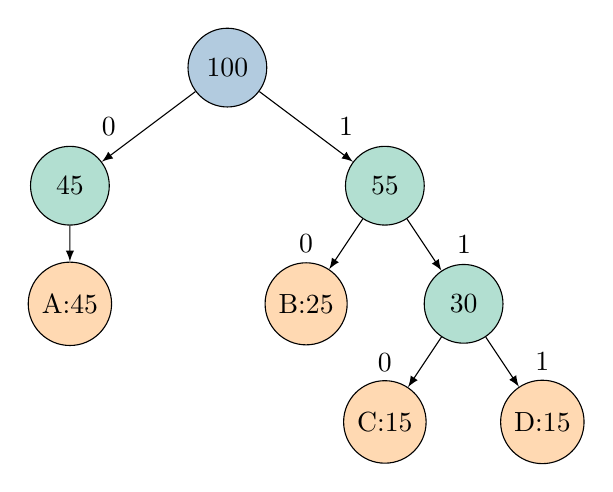
\begin{tikzpicture}[
    level 1/.style={sibling distance=40mm},
    level 2/.style={sibling distance=20mm},
    every node/.style={circle, draw, minimum size=1cm},
    edge from parent/.style={draw, -latex}
]
\node[fill=primaryblue!30] {100}
    child {node[fill=secondarygreen!30] {45}
        child {node[fill=accentorange!30] {A:45}}
        edge from parent node[left, draw=none] {0}
    }
    child {node[fill=secondarygreen!30] {55}
        child {node[fill=accentorange!30] {B:25}
            edge from parent node[left, draw=none] {0}
        }
        child {node[fill=secondarygreen!30] {30}
            child {node[fill=accentorange!30] {C:15}
                edge from parent node[left, draw=none] {0}
            }
            child {node[fill=accentorange!30] {D:15}
                edge from parent node[right, draw=none] {1}
            }
            edge from parent node[right, draw=none] {1}
        }
        edge from parent node[right, draw=none] {1}
    };
\end{tikzpicture}
\caption{Huffman tree for symbols A(45\%), B(25\%), C(15\%), D(15\%)}
\end{figure}
\newpage
\section{Resulting Codes}

\begin{table}[h]
\centering
\begin{tabular}{cccc}
\toprule
\textbf{Symbol} & \textbf{Frequency} & \textbf{Huffman Code} & \textbf{Fixed Code} \\
\midrule
A & 45\% & 0 (1 bit) & 00 (2 bits) \\
B & 25\% & 10 (2 bits) & 01 (2 bits) \\
C & 15\% & 110 (3 bits) & 10 (2 bits) \\
D & 15\% & 111 (3 bits) & 11 (2 bits) \\
\midrule
\textbf{Average} & & \textbf{1.75 bits} & \textbf{2 bits} \\
\bottomrule
\end{tabular}
\caption{Huffman codes vs fixed-length codes}
\end{table}

\section{Algorithm}

\begin{algorithm}[H]
\caption{Huffman Tree Construction}
\begin{algorithmic}[1]
\STATE Create a leaf node for each symbol with its frequency
\STATE Insert all nodes into a min-priority queue $Q$
\WHILE{$|Q| > 1$}
    \STATE Remove two nodes $x, y$ with lowest frequencies
    \STATE Create new node $z$ with $freq(z) = freq(x) + freq(y)$
    \STATE Set $x$ as left child, $y$ as right child of $z$
    \STATE Insert $z$ into $Q$
\ENDWHILE
\RETURN remaining node as root
\end{algorithmic}
\end{algorithm}

\section{Properties}

\begin{itemize}
    \item \textbf{Prefix-free}: No code is a prefix of another
    \item \textbf{Optimal}: Minimum expected code length for symbol-by-symbol encoding
    \item \textbf{Average length}: $L = \sum p_i \cdot l_i$ where $l_i$ is code length
    \item \textbf{Bounded}: $H(X) \leq L < H(X) + 1$ (within 1 bit of entropy)
\end{itemize}

\section{Applications}

\begin{itemize}
    \item \textbf{DEFLATE} (gzip, PNG, ZIP)
    \item \textbf{JPEG} image compression
    \item \textbf{MP3} audio compression
    \item \textbf{Fax machines} (Modified Huffman)
\end{itemize}

% ============================================
% CHAPTER 5: ARITHMETIC CODING
% ============================================
\chapter{Arithmetic Coding}

\section{Overview}

\textbf{Arithmetic coding} encodes an entire message as a single fractional number between 0 and 1. It can achieve compression very close to the theoretical entropy limit.

\begin{itemize}
    \item \textbf{Inventors}: Jorma Rissanen (IBM), Richard Pasco (1976)
    \item \textbf{Type}: Entropy coding (lossless)
    \item \textbf{Advantage}: Can achieve fractional bits per symbol
\end{itemize}

\section{How It Works}

The algorithm progressively narrows an interval based on symbol probabilities:

\begin{figure}[h]
\centering
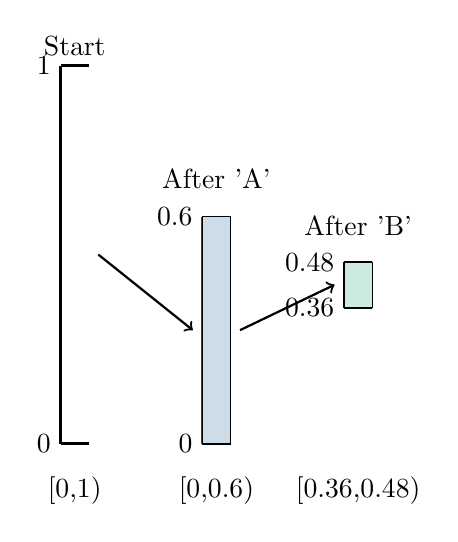
\begin{tikzpicture}[scale=1.2]
    % Initial interval
    \draw[thick] (0,0) -- (0,4);
    \draw[thick] (0,0) -- (0.3,0);
    \draw[thick] (0,4) -- (0.3,4);
    \node[left] at (0,0) {0};
    \node[left] at (0,4) {1};
    \node[above] at (0.15,4) {Start};
    
    % After A (0-0.6)
    \draw[thick, primaryblue] (1.5,0) -- (1.5,2.4);
    \draw[thick] (1.5,0) -- (1.8,0);
    \draw[thick] (1.5,2.4) -- (1.8,2.4);
    \node[left] at (1.5,0) {0};
    \node[left] at (1.5,2.4) {0.6};
    \node[above] at (1.65,2.6) {After 'A'};
    \draw[fill=primaryblue!20] (1.5,0) rectangle (1.8,2.4);
    
    % After B (0.36-0.48)
    \draw[thick, secondarygreen] (3,1.44) -- (3,1.92);
    \draw[thick] (3,1.44) -- (3.3,1.44);
    \draw[thick] (3,1.92) -- (3.3,1.92);
    \node[left] at (3,1.44) {0.36};
    \node[left] at (3,1.92) {0.48};
    \node[above] at (3.15,2.1) {After 'B'};
    \draw[fill=secondarygreen!20] (3,1.44) rectangle (3.3,1.92);
    
    % Arrows
    \draw[->, thick] (0.4,2) -- (1.4,1.2);
    \draw[->, thick] (1.9,1.2) -- (2.9,1.68);
    
    % Labels
    \node at (0.15,-0.5) {[0,1)};
    \node at (1.65,-0.5) {[0,0.6)};
    \node at (3.15,-0.5) {[0.36,0.48)};
\end{tikzpicture}
\caption{Arithmetic coding narrows the interval with each symbol}
\end{figure}

\section{Example: Encoding "AB"}

Given probabilities: A=60\%, B=20\%, C=10\%, D=10\%

\begin{enumerate}
    \item Start with interval [0, 1)
    \item Symbol A: New interval = [0, 0.6)
    \item Symbol B: Within [0, 0.6), B occupies [0.6×0.6, 0.6×0.8) = [0.36, 0.48)
    \item Output: Any number in [0.36, 0.48), e.g., 0.4
\end{enumerate}

\section{Comparison with Huffman}

\begin{table}[h]
\centering
\begin{tabular}{lcc}
\toprule
\textbf{Aspect} & \textbf{Huffman} & \textbf{Arithmetic} \\
\midrule
Bits per symbol & Integer only & Fractional \\
Efficiency & Good & Optimal \\
Complexity & Lower & Higher \\
Adaptation & Needs rebuild & Easy \\
Patent status & Free & Historically patented \\
\bottomrule
\end{tabular}
\caption{Huffman vs Arithmetic coding comparison}
\end{table}

\section{Applications}

\begin{itemize}
    \item \textbf{JPEG} (arithmetic mode, rarely used)
    \item \textbf{H.264/AVC} video (CABAC)
    \item \textbf{JPEG XL}
    \item \textbf{Research} applications
\end{itemize}

% ============================================
% CHAPTER 6: LZ77 AND LZ78
% ============================================
\chapter{LZ77 and LZ78}

\section{Overview}

The \textbf{Lempel-Ziv} algorithms are dictionary-based compression methods that form the foundation of most modern compressors.

\begin{itemize}
    \item \textbf{Inventors}: Abraham Lempel, Jacob Ziv
    \item \textbf{LZ77}: Published 1977 (sliding window)
    \item \textbf{LZ78}: Published 1978 (explicit dictionary)
    \item \textbf{IEEE Milestone}: 2004
\end{itemize}

\section{LZ77: Sliding Window}

LZ77 uses a sliding window to find repeated patterns and replaces them with (offset, length) pairs.

\begin{figure}[h]
\centering
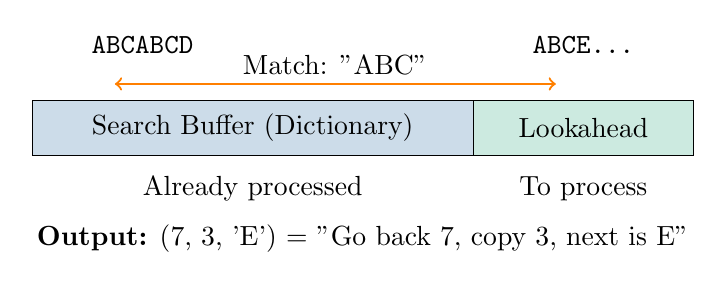
\begin{tikzpicture}[scale=0.7]
    % Search buffer
    \draw[fill=primaryblue!20] (0,0) rectangle (8,1);
    \node at (4,0.5) {Search Buffer (Dictionary)};
    \node[below] at (4,-0.2) {Already processed};
    
    % Lookahead buffer
    \draw[fill=secondarygreen!20] (8,0) rectangle (12,1);
    \node at (10,0.5) {Lookahead};
    \node[below] at (10,-0.2) {To process};
    
    % Sample text
    \node at (2,2) {\texttt{ABCABCD}};
    \node at (10,2) {\texttt{ABCE...}};
    
    % Match arrow
    \draw[<->, thick, accentorange] (1.5,1.3) -- (9.5,1.3);
    \node[above] at (5.5,1.3) {Match: "ABC"};
    
    % Output
    \node at (6,-1.5) {\textbf{Output:} (7, 3, 'E') = "Go back 7, copy 3, next is E"};
\end{tikzpicture}
\caption{LZ77 sliding window compression}
\end{figure}

\section{LZ77 Output Format}

Each output token contains:
\begin{itemize}
    \item \textbf{Offset}: Distance back to the match
    \item \textbf{Length}: Number of characters to copy
    \item \textbf{Next}: The character following the match
\end{itemize}

\begin{table}[h]
\centering
\begin{tabular}{lccc}
\toprule
\textbf{Input} & \textbf{Offset} & \textbf{Length} & \textbf{Next} \\
\midrule
A & 0 & 0 & A \\
B & 0 & 0 & B \\
ABAB & 2 & 2 & A \\
\bottomrule
\end{tabular}
\caption{LZ77 encoding example for "ABABAB"}
\end{table}

\section{LZ78: Explicit Dictionary}

LZ78 builds an explicit dictionary of phrases encountered during compression.

\begin{algorithm}[H]
\caption{LZ78 Encoding}
\begin{algorithmic}[1]
\STATE Initialize dictionary with empty string at index 0
\STATE $phrase \gets$ empty
\WHILE{input not empty}
    \STATE Read next symbol $c$
    \IF{$phrase + c$ is in dictionary}
        \STATE $phrase \gets phrase + c$
    \ELSE
        \STATE Output (index of $phrase$, $c$)
        \STATE Add $phrase + c$ to dictionary
        \STATE $phrase \gets$ empty
    \ENDIF
\ENDWHILE
\end{algorithmic}
\end{algorithm}

\section{Comparison}

\begin{table}[h]
\centering
\begin{tabular}{lcc}
\toprule
\textbf{Aspect} & \textbf{LZ77} & \textbf{LZ78} \\
\midrule
Dictionary & Implicit (window) & Explicit \\
Memory & Fixed window size & Grows with input \\
Decompression & Must start at beginning & Can be random access \\
Foundation for & DEFLATE, gzip & LZW, GIF \\
\bottomrule
\end{tabular}
\caption{LZ77 vs LZ78 comparison}
\end{table}

% ============================================
% CHAPTER 7: LZW
% ============================================
\chapter{LZW (Lempel-Ziv-Welch)}

\section{Overview}

\textbf{LZW} is an improvement of LZ78 that doesn't need to output the next character, making it more efficient.

\begin{itemize}
    \item \textbf{Inventor}: Terry Welch (1984)
    \item \textbf{Type}: Dictionary-based lossless
    \item \textbf{Patent}: Expired 2003 (US), 2004 (international)
\end{itemize}

\section{How It Works}

\begin{enumerate}
    \item Initialize dictionary with all single characters
    \item Find longest string $W$ in dictionary that matches input
    \item Output dictionary index for $W$
    \item Add $W$ + next character to dictionary
    \item Repeat from step 2
\end{enumerate}

\section{Example: Encoding "ABABAB"}

\begin{table}[h]
\centering
\begin{tabular}{ccccc}
\toprule
\textbf{Step} & \textbf{Current} & \textbf{Next} & \textbf{Output} & \textbf{Add to Dict} \\
\midrule
1 & A & B & 65 (A) & 256 = AB \\
2 & B & A & 66 (B) & 257 = BA \\
3 & AB & A & 256 (AB) & 258 = ABA \\
4 & AB & - & 256 (AB) & - \\
\bottomrule
\end{tabular}
\caption{LZW encoding steps for "ABABAB"}
\end{table}

Initial dictionary: A=65, B=66, ..., Z=90

Output: 65, 66, 256, 256 (4 codes instead of 6 characters)

\section{Decoding}

The decoder rebuilds the dictionary in the same way:

\begin{enumerate}
    \item Initialize dictionary with single characters
    \item Read code, output corresponding string
    \item Add previous string + first char of current string to dictionary
\end{enumerate}

\section{Applications}

\begin{itemize}
    \item \textbf{GIF} image format
    \item \textbf{TIFF} (optional compression)
    \item \textbf{PDF} (optional)
    \item \textbf{Unix compress} utility (.Z files)
\end{itemize}

% ============================================
% CHAPTER 8: DEFLATE
% ============================================
\chapter{DEFLATE}

\section{Overview}

\textbf{DEFLATE} combines LZ77 and Huffman coding to achieve good compression with reasonable speed. It's one of the most widely used compression algorithms.

\begin{itemize}
    \item \textbf{Inventor}: Phil Katz (PKZIP, 1990)
    \item \textbf{Standard}: RFC 1951 (1996)
    \item \textbf{Type}: Hybrid (LZ77 + Huffman)
\end{itemize}

\section{Algorithm Pipeline}

\begin{figure}[h]
\centering
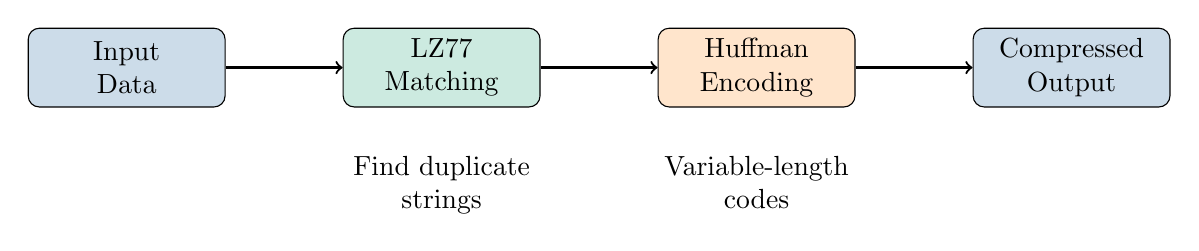
\begin{tikzpicture}[
    box/.style={draw, rounded corners, minimum width=2.5cm, minimum height=1cm, align=center},
    arrow/.style={->, thick}
]
    \node[box, fill=primaryblue!20] (input) at (0,0) {Input\\Data};
    \node[box, fill=secondarygreen!20] (lz77) at (4,0) {LZ77\\Matching};
    \node[box, fill=accentorange!20] (huffman) at (8,0) {Huffman\\Encoding};
    \node[box, fill=primaryblue!20] (output) at (12,0) {Compressed\\Output};
    
    \draw[arrow] (input) -- (lz77);
    \draw[arrow] (lz77) -- (huffman);
    \draw[arrow] (huffman) -- (output);
    
    \node[below, align=center] at (4,-1) {Find duplicate\\strings};
    \node[below, align=center] at (8,-1) {Variable-length\\codes};
\end{tikzpicture}
\caption{DEFLATE compression pipeline}
\end{figure}

\section{Step 1: LZ77 Compression}

\begin{itemize}
    \item Window size: 32 KB
    \item Match length: 3-258 bytes
    \item Outputs: Literals and (length, distance) pairs
\end{itemize}

\section{Step 2: Huffman Coding}

Two Huffman trees are used:
\begin{enumerate}
    \item \textbf{Literal/Length tree}: Encodes literals (0-255), end-of-block (256), and lengths (257-285)
    \item \textbf{Distance tree}: Encodes distances (0-29 with extra bits)
\end{enumerate}

\section{Block Types}

\begin{table}[h]
\centering
\begin{tabular}{clp{6cm}}
\toprule
\textbf{Code} & \textbf{Type} & \textbf{Description} \\
\midrule
00 & Stored & No compression, raw data \\
01 & Static & Pre-defined Huffman trees \\
10 & Dynamic & Custom Huffman trees included \\
11 & Reserved & Not used \\
\bottomrule
\end{tabular}
\caption{DEFLATE block types}
\end{table}

\section{Compression Levels}

\begin{table}[h]
\centering
\begin{tabular}{ccc}
\toprule
\textbf{Level} & \textbf{Speed} & \textbf{Compression} \\
\midrule
0 & Fastest & None (store only) \\
1-3 & Fast & Low \\
4-6 & Balanced & Medium \\
7-9 & Slow & High \\
\bottomrule
\end{tabular}
\caption{DEFLATE compression levels}
\end{table}

\section{Applications}

\begin{itemize}
    \item \textbf{gzip} (.gz files)
    \item \textbf{ZIP} archives
    \item \textbf{PNG} images
    \item \textbf{HTTP compression}
    \item \textbf{PDF} (FlateDecode)
\end{itemize}

% ============================================
% CHAPTER 9: MODERN ALGORITHMS
% ============================================
\chapter{Modern Compression Algorithms}

\section{LZ4}

\textbf{LZ4} is an extremely fast compression algorithm focused on speed over compression ratio.

\begin{itemize}
    \item \textbf{Author}: Yann Collet
    \item \textbf{Focus}: Speed
    \item \textbf{Compression}: ~500 MB/s
    \item \textbf{Decompression}: ~3000 MB/s
\end{itemize}

\textbf{Key features}:
\begin{itemize}
    \item No entropy coding (simpler, faster)
    \item Small dictionary
    \item Used in: Linux kernel, ZFS, MySQL
\end{itemize}

\section{Zstandard (zstd)}

\textbf{Zstandard} combines high compression ratios with excellent speed.

\begin{itemize}
    \item \textbf{Author}: Yann Collet (Facebook, 2016)
    \item \textbf{Standard}: RFC 8478
    \item \textbf{Levels}: -7 to 22
\end{itemize}

\begin{figure}[h]
\centering
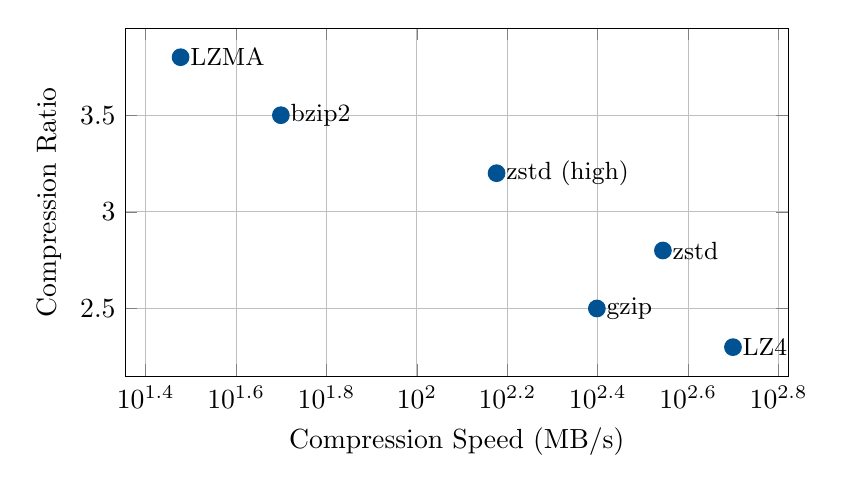
\begin{tikzpicture}
\begin{axis}[
    xlabel={Compression Speed (MB/s)},
    ylabel={Compression Ratio},
    xmode=log,
    legend pos=north east,
    grid=major,
    width=10cm,
    height=6cm
]
\addplot[only marks, mark=*, color=primaryblue, mark size=3pt] coordinates {
    (250, 2.5) % gzip
    (500, 2.3) % LZ4
    (350, 2.8) % zstd default
    (150, 3.2) % zstd high
    (50, 3.5) % bzip2
    (30, 3.8) % LZMA
};
\node[right] at (axis cs:250, 2.5) {\small gzip};
\node[right] at (axis cs:500, 2.3) {\small LZ4};
\node[right] at (axis cs:350, 2.8) {\small zstd};
\node[right] at (axis cs:150, 3.2) {\small zstd (high)};
\node[right] at (axis cs:50, 3.5) {\small bzip2};
\node[right] at (axis cs:30, 3.8) {\small LZMA};
\end{axis}
\end{tikzpicture}
\caption{Compression algorithms: Speed vs Ratio comparison}
\end{figure}
\newpage
\section{Brotli}

\textbf{Brotli} is optimized for web content, offering better compression than gzip.

\begin{itemize}
    \item \textbf{Authors}: Google (Alakuijala, Szabadka, 2013)
    \item \textbf{Standard}: RFC 7932 (2016)
    \item \textbf{Features}: 120 KB static dictionary, context modeling
\end{itemize}

\textbf{Web improvements over gzip}:
\begin{itemize}
    \item JavaScript: $\sim$15\% smaller
    \item HTML: $\sim$20\% smaller
    \item CSS: $\sim$16\% smaller
\end{itemize}

\section{bzip2}

\textbf{bzip2} uses the Burrows-Wheeler Transform for high compression.

\begin{figure}[h]
\centering
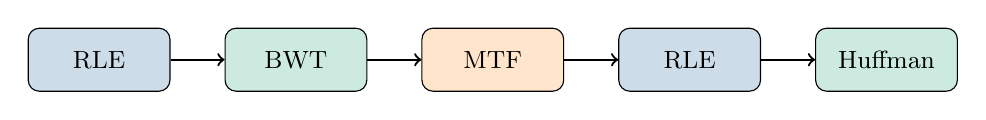
\begin{tikzpicture}[
    box/.style={draw, rounded corners, minimum width=1.8cm, minimum height=0.8cm, align=center, font=\small},
    arrow/.style={->, thick}
]
    \node[box, fill=primaryblue!20] (rle1) at (0,0) {RLE};
    \node[box, fill=secondarygreen!20] (bwt) at (2.5,0) {BWT};
    \node[box, fill=accentorange!20] (mtf) at (5,0) {MTF};
    \node[box, fill=primaryblue!20] (rle2) at (7.5,0) {RLE};
    \node[box, fill=secondarygreen!20] (huff) at (10,0) {Huffman};
    
    \draw[arrow] (rle1) -- (bwt);
    \draw[arrow] (bwt) -- (mtf);
    \draw[arrow] (mtf) -- (rle2);
    \draw[arrow] (rle2) -- (huff);
\end{tikzpicture}
\caption{bzip2 compression pipeline}
\end{figure}

\section{LZMA/7z}

\textbf{LZMA} achieves the highest compression ratios among common algorithms.

\begin{itemize}
    \item \textbf{Author}: Igor Pavlov (7-Zip, 1998)
    \item \textbf{Features}: Large dictionary (up to 4 GB), range coding
    \item \textbf{Trade-off}: Slow compression, fast decompression
\end{itemize}

\section{Snappy}

\textbf{Snappy} prioritizes speed for database and big data applications.

\begin{itemize}
    \item \textbf{Author}: Google (2011)
    \item \textbf{Compression}: $\sim$250 MB/s
    \item \textbf{Decompression}: $\sim$500 MB/s
    \item \textbf{Used in}: BigTable, MongoDB, Cassandra
\end{itemize}

% ============================================
% CHAPTER 10: COMPARISON
% ============================================
\chapter{Algorithm Comparison}

\section{Performance Summary}

\begin{table}[h]
\centering
\small
\begin{tabular}{lcccc}
\toprule
\textbf{Algorithm} & \textbf{Type} & \textbf{Compress} & \textbf{Decompress} & \textbf{Ratio} \\
\midrule
LZ4 & Dictionary & Very Fast & Very Fast & Low \\
Snappy & Dictionary & Very Fast & Very Fast & Low \\
gzip/DEFLATE & Hybrid & Medium & Fast & Medium \\
Brotli & Hybrid & Medium & Fast & High \\
zstd & Hybrid & Fast & Fast & High \\
bzip2 & Block-sort & Slow & Medium & High \\
LZMA/7z & Dictionary & Very Slow & Medium & Very High \\
\bottomrule
\end{tabular}
\caption{Compression algorithms performance comparison}
\end{table}

\section{Use Case Recommendations}

\begin{table}[h]
\centering
\begin{tabular}{lp{8cm}}
\toprule
\textbf{Use Case} & \textbf{Recommended Algorithm} \\
\midrule
Real-time compression & LZ4, Snappy \\
Web content & Brotli, zstd \\
General archiving & zstd, gzip \\
Maximum compression & LZMA, bzip2 \\
Text files & bzip2, LZMA \\
Database storage & LZ4, Snappy, zstd \\
Streaming data & LZ4, zstd \\
\bottomrule
\end{tabular}
\caption{Algorithm recommendations by use case}
\end{table}

\section{Historical Timeline}

\begin{figure}[h]
\centering
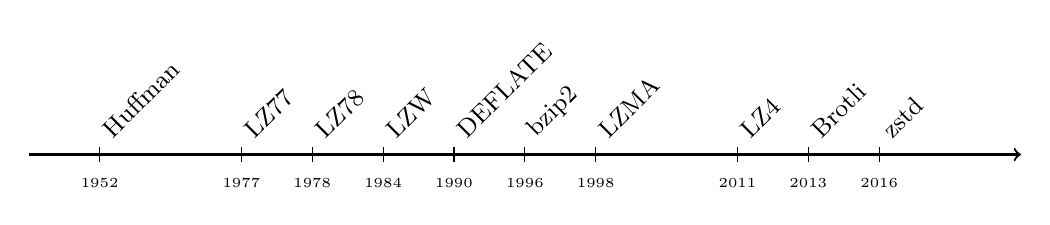
\begin{tikzpicture}[scale=0.9]
    % Timeline
    \draw[thick, ->] (0,0) -- (14,0);
    
    % Years and algorithms
    \foreach \x/\year/\algo in {
        1/1952/Huffman,
        3/1977/LZ77,
        4/1978/LZ78,
        5/1984/LZW,
        6/1990/DEFLATE,
        7/1996/bzip2,
        8/1998/LZMA,
        10/2011/LZ4,
        11/2013/Brotli,
        12/2016/zstd
    } {
        \draw (\x,0.1) -- (\x,-0.1);
        \node[below, font=\tiny] at (\x,-0.2) {\year};
        \node[above, rotate=45, anchor=west, font=\small] at (\x,0.2) {\algo};
    }
\end{tikzpicture}
\caption{Evolution of compression algorithms}
\end{figure}

% ============================================
% CHAPTER 11: CONCLUSION
% ============================================
\chapter{Conclusion}

\section{Key Takeaways}

\begin{enumerate}
    \item \textbf{No single best algorithm}: The choice depends on speed, ratio, and use case requirements.
    
    \item \textbf{Trade-offs}: Higher compression generally means slower speed.
    
    \item \textbf{Modern algorithms}: Zstandard offers the best balance for most applications.
    
    \item \textbf{Specialized use cases}: LZ4/Snappy for databases, Brotli for web, LZMA for archives.
\end{enumerate}

\section{Decision Flowchart}

\begin{figure}[h]
\centering
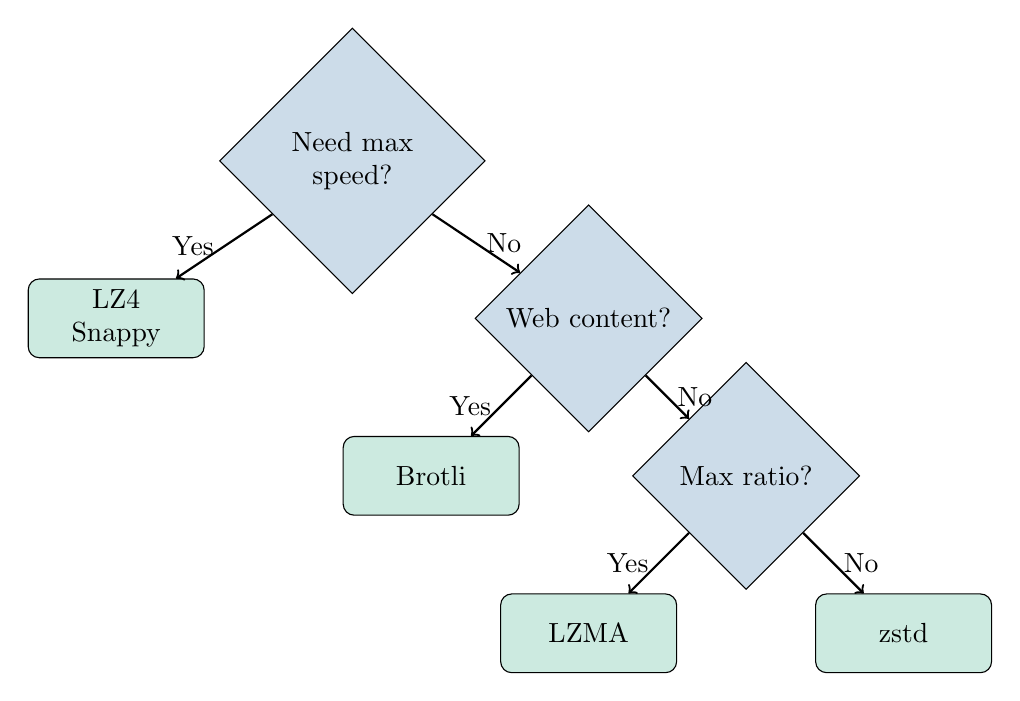
\begin{tikzpicture}[
    decision/.style={diamond, draw, fill=primaryblue!20, text width=2.5cm, align=center, inner sep=1pt},
    block/.style={rectangle, draw, fill=secondarygreen!20, rounded corners, text width=2cm, align=center, minimum height=1cm},
    arrow/.style={->, thick}
]
    \node[decision] (speed) at (0,0) {Need max speed?};
    \node[block] (lz4) at (-3,-2) {LZ4\\Snappy};
    \node[decision] (web) at (3,-2) {Web content?};
    \node[block] (brotli) at (1,-4) {Brotli};
    \node[decision] (ratio) at (5,-4) {Max ratio?};
    \node[block] (lzma) at (3,-6) {LZMA};
    \node[block] (zstd) at (7,-6) {zstd};
    
    \draw[arrow] (speed) -- node[left] {Yes} (lz4);
    \draw[arrow] (speed) -- node[right] {No} (web);
    \draw[arrow] (web) -- node[left] {Yes} (brotli);
    \draw[arrow] (web) -- node[right] {No} (ratio);
    \draw[arrow] (ratio) -- node[left] {Yes} (lzma);
    \draw[arrow] (ratio) -- node[right] {No} (zstd);
\end{tikzpicture}
\caption{Algorithm selection decision tree}
\end{figure}

\section{Future Trends}

\begin{itemize}
    \item \textbf{Hardware acceleration}: GPU and FPGA-based compression
    \item \textbf{Machine learning}: Neural network-based compression
    \item \textbf{Adaptive algorithms}: Context-aware compression
    \item \textbf{Quantum-resistant}: Compression with post-quantum security
\end{itemize}

% ============================================
% BIBLIOGRAPHY
% ============================================
\chapter*{References}
\addcontentsline{toc}{chapter}{References}

\begin{enumerate}
    \item Huffman, D. A. (1952). ``A Method for the Construction of Minimum-Redundancy Codes.'' \textit{Proceedings of the IRE}.
    
    \item Ziv, J., Lempel, A. (1977). ``A Universal Algorithm for Sequential Data Compression.'' \textit{IEEE Trans. Information Theory}.
    
    \item Ziv, J., Lempel, A. (1978). ``Compression of Individual Sequences via Variable-Rate Coding.'' \textit{IEEE Trans. Information Theory}.
    
    \item Welch, T. (1984). ``A Technique for High-Performance Data Compression.'' \textit{Computer}.
    
    \item RFC 1951 (1996). ``DEFLATE Compressed Data Format Specification.''
    
    \item RFC 7932 (2016). ``Brotli Compressed Data Format.''
    
    \item RFC 8478 (2018). ``Zstandard Compression and the application/zstd Media Type.''
    
    \item Salomon, D. (2007). \textit{Data Compression: The Complete Reference} (4th ed.). Springer.
    
    \item Seward, J. ``bzip2 and libbzip2 Documentation.'' sourceware.org.
    
    \item Collet, Y. ``LZ4 and Zstandard Documentation.'' github.com/facebook.
\end{enumerate}

\end{document}
